\documentclass{beamer}

\mode<presentation>
{
  \usetheme{default}
  \usecolortheme{default}
  \usefonttheme{default}
  \setbeamertemplate{navigation symbols}{}
  \setbeamertemplate{caption}[numbered]
  \setbeamertemplate{footline}[page number]
  \setbeamercolor{frametitle}{fg=white}
  \setbeamercolor{footline}{fg=black}
} 

\usepackage[english]{babel}
\usepackage[utf8x]{inputenc}
\usepackage{tikz}
\usepackage{listings}
\usepackage{courier}
\usepackage{array}
\usepackage{bold-extra}
\usepackage{minted}
\usepackage{ulem}
\usepackage{xpatch}
\usepackage{fancyvrb}

\xdefinecolor{darkblue}{rgb}{0.1,0.1,0.7}
\xdefinecolor{darkgreen}{rgb}{0,0.5,0}
\xdefinecolor{darkgrey}{rgb}{0.35,0.35,0.35}
\xdefinecolor{darkorange}{rgb}{0.8,0.5,0}
\xdefinecolor{darkred}{rgb}{0.7,0,0}
\xdefinecolor{dianablue}{rgb}{0.18,0.24,0.31}
\definecolor{commentgreen}{rgb}{0,0.6,0}
\definecolor{stringmauve}{rgb}{0.58,0,0.82}

\lstset{ %
  backgroundcolor=\color{white},      % choose the background color
  basicstyle=\ttfamily\small,         % size of fonts used for the code
  breaklines=true,                    % automatic line breaking only at whitespace
  captionpos=b,                       % sets the caption-position to bottom
  commentstyle=\color{commentgreen},  % comment style
  escapeinside={\%*}{*)},             % if you want to add LaTeX within your code
  keywordstyle=\color{blue},          % keyword style
  stringstyle=\color{stringmauve},    % string literal style
  showstringspaces=false,
  showlines=true
}

\lstdefinelanguage{scala}{
  morekeywords={abstract,case,catch,class,def,%
    do,else,extends,false,final,finally,%
    for,if,implicit,import,match,mixin,%
    new,null,object,override,package,%
    private,protected,requires,return,sealed,%
    super,this,throw,trait,true,try,%
    type,val,var,while,with,yield},
  otherkeywords={=>,<-,<\%,<:,>:,\#,@},
  sensitive=true,
  morecomment=[l]{//},
  morecomment=[n]{/*}{*/},
  morestring=[b]",
  morestring=[b]',
  morestring=[b]"""
}

\title[2017-08-22-acat-hepquery]{Toward real-time data query systems in HEP}
\author{Jim Pivarski}
\institute{Princeton University -- DIANA}
\date{August 22, 2017}

\xpatchcmd{\sout}
  {\bgroup}
  {\bgroup\def\ULthickness{1.5 pt}}
  {}{}

\begin{document}

\logo{\pgfputat{\pgfxy(0.11, 8)}{\pgfbox[right,base]{\tikz{\filldraw[fill=dianablue, draw=none] (0 cm, 0 cm) rectangle (50 cm, 1 cm);}}}\pgfputat{\pgfxy(0.11, -0.6)}{\pgfbox[right,base]{\tikz{\filldraw[fill=dianablue, draw=none] (0 cm, 0 cm) rectangle (50 cm, 1 cm);}
\includegraphics[height=0.99 cm]{diana-hep-logo.png}\tikz{\filldraw[fill=dianablue, draw=none] (0 cm, 0 cm) rectangle (4.9 cm, 1 cm);}}}}

\begin{frame}
  \titlepage
\end{frame}

\logo{\pgfputat{\pgfxy(0.11, 8)}{\pgfbox[right,base]{\tikz{\filldraw[fill=dianablue, draw=none] (0 cm, 0 cm) rectangle (50 cm, 1 cm);}
\includegraphics[height=1 cm]{diana-hep-logo.png}}}}

% Uncomment these lines for an automatically generated outline.
%\begin{frame}{Outline}
%  \tableofcontents
%\end{frame}

%%%%%%%%%%%%%%%%%%%%%%%%%%%%%%%%%%%%%%%%%%%%%%%%%%%%%%%

\begin{frame}{The dream}
\vspace{0.5 cm}
LHC experiments are pretty efficient at data handling up to Analysis Object Datasets (AODs), but AODs to final plots is a wild west of hacky scripts, unnecessary copying, and wasted resources.

\vspace{0.2 cm}
\only<1>{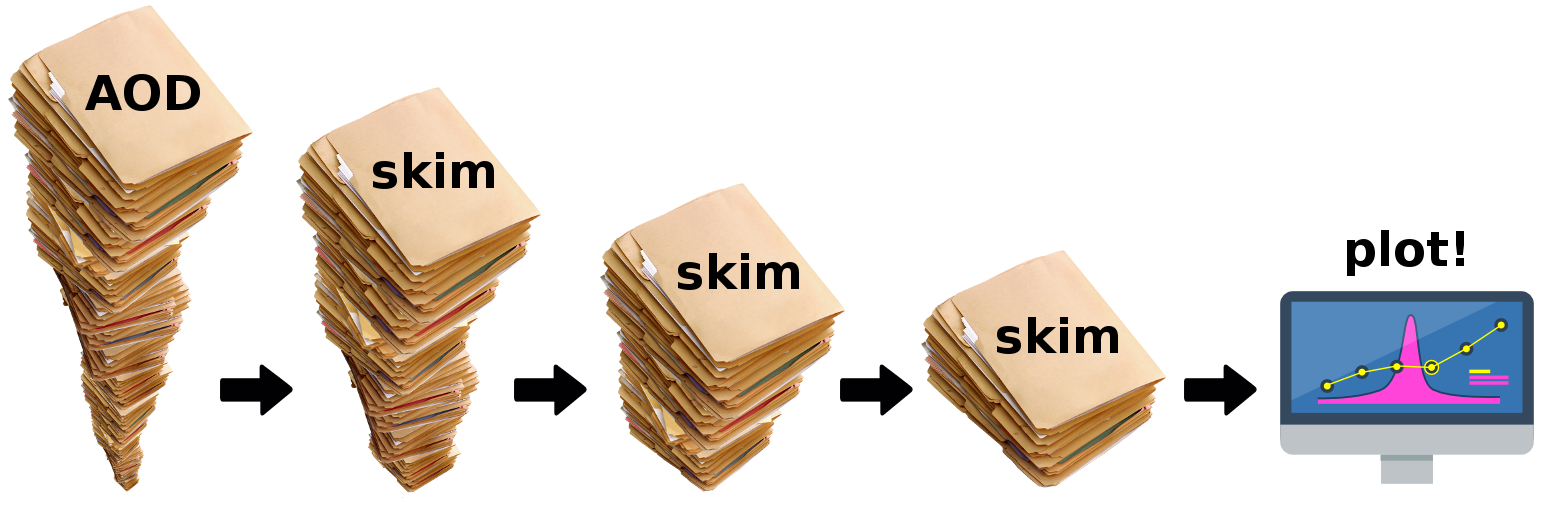
\includegraphics[width=\linewidth]{stack-of-files.png}}\only<2>{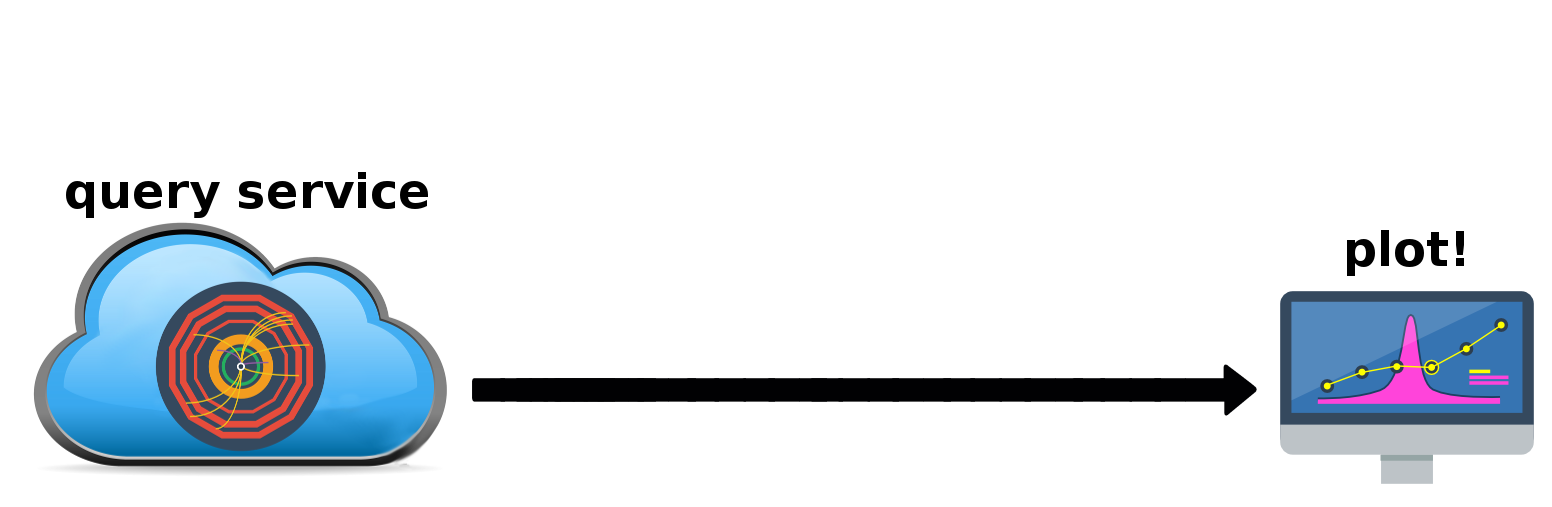
\includegraphics[width=\linewidth]{stack-of-files-2.png}}

\vspace{0.5 cm}
\begin{uncoverenv}<2>
Ideally, we'd want to turn AOD directly into plots, quickly enough for interactive analysis (seconds per scan at most).
\end{uncoverenv}
\end{frame}

\begin{frame}{Why this is a Good Thing}
\large
\vspace{0.5 cm}
\begin{itemize}\setlength{\itemsep}{0.5 cm}
\item Users would plot the data before doing anything else.

\vspace{0.2 cm}
\textcolor{gray}{\normalsize (Skims for maximum likelihood fits, etc.\ should be possible, but can be more streamlined {\it after} exploratory plotting.)}

\vspace{-0.2 cm}
\item Focus on physics and statistical issues, not data handling.
\item Centralization facilitates provenance and reproducibility.
\item Shared CPU, disk, and memory is more efficient.
\item Small institutions would not be ``priced out'' of analysis for lack of resources to copy and locally process the data.
\end{itemize}
\end{frame}

\begin{frame}{Existence proof}

In some industries, it is possible to ``process petabyes of data and trillions of records in seconds\footnotemark[1],'' usually as SQL.

\vspace{0.2 cm}
In fact, there are many low-latency query server engines available, mostly open source.

\vspace{0.5 cm}
\mbox{\hspace{-1 cm}

\includegraphics[height=1.23 cm]{drill-logo.png}

\includegraphics[height=1.23 cm]{impala-logo.png}

\includegraphics[height=1.23 cm]{kudu-logo.png}

\includegraphics[height=1.23 cm]{ibis-logo.png}

\includegraphics[height=1.23 cm]{hawk-logo.png}

\includegraphics[height=1.23 cm]{dremel-logo.png}

\includegraphics[height=1.23 cm]{bigquery-logo.png}

\includegraphics[height=1.23 cm]{sparksql-logo.png}}

\vspace{0.5 cm}
\begin{uncoverenv}<2>
Apache Drill comes closest to fitting our needs, but it's
\begin{itemize}
\item SQL (not expressive enough for HEP)
\item Java (hard to link to HEP software)
\item more suited to ``flat ntuple'' analysis (see next slides).
\end{itemize}
\end{uncoverenv}

\footnotetext[1]{\textcolor{blue}{\url{https://wiki.apache.org/incubator/DrillProposal}}}
\end{frame}

%% \begin{frame}{Existence proof}
%% \vspace{0.5 cm}
%% \mbox{ } \hfill 
\includegraphics[height=2 cm]{drill-logo.png} \hfill \mbox{ }

%% \begin{columns}
%% \column{0.5\linewidth}
%% \textcolor{darkblue}{\large \underline{What's right}}

%% \begin{itemize}
%% \item lightweight parallelization
%% \item columnar data
%% \item just-in-time (JIT) compilation, vectorization
%% \item data stay on the server, only summaries come down
%% \item extensible: plug-in architecture
%% \end{itemize}

%% \column{0.5\linewidth}
%% \textcolor{darkblue}{\large \underline{What's wrong}}

%% \begin{itemize}
%% \item SQL isn't expressive enough for physics analysis
%% \item Drill's query planning optimizations are based on SQL's structure
%% \item Drill's native Java is foreign to most of our ecosystem in HEP
%% \end{itemize}

%% \end{columns}

%% \vspace{0.5 cm}
%% \end{frame}

%% \vspace{0.5 cm}
%% Either extend every part of Drill or build a query system with a similar architecture using the same tools (e.g.\ Zookeeper).

\begin{frame}{Toward a query system for HEP}
\vspace{0.5 cm}
\large This talk is about what we would need to make (or alter) a query system for HEP analysis:

\vspace{0.3 cm}
\begin{itemize}\setlength{\itemsep}{0.3 cm}
\item {\bf fast execution} on {\it nested, non-flat} data
\item {\bf distributed processing:} caching and data locality, uneven and changing dataset popularity, aggregation
\item \sout{{\bf HEP-specific query language}} (in the abstract for this talk, but I'm going to focus more on the above)
\end{itemize}
\end{frame}

\begin{frame}
\begin{center}
\huge \textcolor{darkblue}{Fast execution}
\end{center}
\end{frame}

\begin{frame}{The core issue}
\vspace{0.5 cm}
SQL-like query engines are optimized for what we'd call a ``flat ntuple analysis''--- rectangular table of numbers, sliced, filtered, aggregated, and joined.

\vspace{0.5 cm}
\uncover<2->{Only late-stage HEP analysis could fit this model, not AOD.}

\vspace{0.5 cm}
\uncover<3->{General physics analysis requires arbitrary-length lists of objects: e.g.\ events containing jets containing tracks containing hits.}

\vspace{0.5 cm}
\uncover<4->{But frameworks that create physics objects at runtime would be slow to process as queries.}
\end{frame}

\begin{frame}{Illustration}
\vspace{0.5 cm}

\large \textcolor{darkblue}{\underline{Query: fill a histogram with jet $p_T$ of all jets.}}

\begin{center}
\renewcommand{\arraystretch}{1.5}
\small
\begin{tabular}{r l}
\large 0.018 MHz & \large full CMS framework (single-threaded C++) \\
\uncover<5->{\large 0.029 MHz & \large load all 95 jet branches in ROOT} \\
\uncover<4->{\large 2.8 MHz & \large load jet $p_T$ branch (and no others) in ROOT} \\
\uncover<3->{\large 12 MHz & \large allocate C++ objects on heap, fill, delete} \\
\uncover<2->{\large 31 MHz & \large allocate C++ objects on stack, fill histogram} \\
\large 250 MHz & \large minimal ``for'' loop (single-threaded C) \\
\end{tabular}
\end{center}

\uncover<6->{\large \textcolor{darkblue}{Four orders of magnitude in performance lost to provide an object-oriented view of the jets, with all attributes filled.}}
\end{frame}

\begin{frame}[fragile]{Alternative}
\vspace{0.5 cm}
\fbox{\begin{minipage}{\linewidth}
Instead of deserializing data into objects, translate the code into loops over raw arrays.
\end{minipage}}

\vspace{0.25 cm}
\textcolor{darkblue}{\underline{User writes code with ``event'' and ``jet'' objects:}}

\scriptsize
\begin{minted}{python}
histogram = numpy.zeros(100, dtype=numpy.int32)

def fcn(roottree, histogram):
    for event in roottree:
        for jet in event.jets:
            bin = int(jet.pt)
            if bin >= 0 and bin < 100:
                histogram[bin] += 1
\end{minted}

\vspace{0.25 cm}
\textcolor{darkblue}{\normalsize \underline{which are translated into indexes over raw arrays:}}

\scriptsize
\begin{minted}{c++}
void fcn(int* events, int* jets, float* jetptdata, int* histogram) {
    int event, jet;
    for (event = 0;  event < events[1];  event++)
        for (jet = jets[event];  jet < jets[event + 1];  jet++) {
            int bin = (int)jetptdata[jet];
            if (bin >= 0  &&  bin < 100)
                histogram[bin] += 1;
}}
\end{minted}

\end{frame}

\begin{frame}[fragile]{Result}
\vspace{0.5 cm}
\hspace{-0.75 cm}\begin{minipage}{\linewidth}\scriptsize
\begin{Verbatim}[commandchars=\\\{\}]
 97% done; reading: 262.094 MB/s, computing: 66.308 MHz (...TeV_2_7.root)
 98% done; reading: 337.129 MB/s, computing: 67.579 MHz (...TeV_2_8.root)
100% done; reading: 232.974 MB/s, computing: 67.133 MHz (...TeV_2_9.root)
========================================================================================
total time spent compiling: 0.353 sec
             opening files: 0.078 sec
              reading data: 0.238 sec (46.302 MB --> 194.745 MB/s)
                 computing: 0.061 sec (5389283 entries --> \textcolor{red}{87.645 MHz})

      from start to finish: 0.734 sec
\end{Verbatim}
\end{minipage}

\vspace{1 cm}
Object-oriented calculations can now be performed \mbox{at \textcolor{red}{$\mathcal{O}(\mbox{100 MHz})$}.\hspace{-0.5 cm}}

\vspace{0.25 cm}
Disk reads and RAM strides are more sequential than if they were chasing pointers.

\vspace{0.25 cm}
No need for ``schema evolution'' because data \mbox{never get deserialized.\hspace{-0.25 cm}} Different versions of a dataset can share column arrays, reducing disk space of revisions. Popular columns should be cached.
\end{frame}

%% \begin{frame}[fragile]{More complex example}
%% \vspace{0.5 cm}
%% This straightforward nested loop would be very difficult to express in SQL.

%% \vspace{0.25 cm}
%% The ``event'', ``mu1'', and ``mu2'' objects are replaced with array lookups at runtime.

%% \scriptsize
%% \begin{minted}{python}
%% for event in roottree:
%%     for i in range(len(event.muons)):      # don't repeat muons!
%%         for j in range(i + 1, len(event.muons)):
%%             mu1 = event.muons[i]
%%             mu2 = event.muons[j]
%%             mass = sqrt(2 * mu1.pt * mu2.pt *
%%                         (cosh(mu1.eta - mu2.eta) - cos(mu1.phi - mu2.phi)))
%% \end{minted}
%% \end{frame}

\begin{frame}{You can try this out}
Our PLUR library\footnotemark[1] puts {\bf P}rimitive, {\bf L}ist, {\bf U}nion, and {\bf R}ecord data into flat arrays and translates Python code to do array lookups.

\vspace{0.5 cm}
The translated Python is then compiled by Numba\footnotemark[2] (Python compiler for numerical algorithms) into fast bytecode.

\vspace{0.5 cm}
Our contributions to ROOT\footnotemark[3] allow ROOT TBranch data to be rapidly viewed as Numpy arrays ($10\times$ faster than root\_numpy).

\vspace{0.5 cm}
This is being gathered into a HEPQuery application\footnotemark[4] to provide a query service. See the READMEs for more realistic examples.

\footnotetext[1]{\textcolor{blue}{\url{https://github.com/diana-hep/plur}}}
\footnotetext[2]{\textcolor{blue}{\url{http://numba.pydata.org/}}}
\footnotetext[3]{\textcolor{blue}{\url{https://jpivarski.github.io/devlog-tbranch-numpy/}}}
\footnotetext[4]{\textcolor{blue}{\url{https://github.com/diana-hep/hepquery/}}}
\end{frame}

\begin{frame}
\begin{center}
\huge \textcolor{darkblue}{Distributed processing}
\end{center}
\end{frame}

\begin{frame}{Challenges}
\vspace{0.5 cm}
\textcolor{darkblue}{Two types of query:}
\begin{itemize}
\item transform an input dataset into an output dataset, both of which live on the server;
\item aggregate an input dataset into histograms, which are returned to the user's terminal.
\end{itemize}

\vspace{0.5 cm}
\uncover<2->{Aggregations require two phases: splitting into subtasks (map) and combining partial results (reduce). These must be coordinated.}

\vspace{0.5 cm}
\uncover<3->{Input data should be cached with column-granularity.}

\vspace{0.5 cm}
\uncover<4->{Subtasks should {\it preferentially} be sent where their input data are cached (for data locality), but not {\it exclusively} (to elastically scale with dataset popularity).}
\end{frame}

\begin{frame}{Distributed state}
\vspace{0.5 cm}
To track ongoing jobs, accumulate partial histograms, and know where to find cached inputs, the query server will need to have mutable state.

\vspace{0.3 cm}
\begin{uncoverenv}<2->
\hfill 
\includegraphics[height=1.2 cm]{zookeeper.png} 
\includegraphics[height=1.2 cm]{mongodb.png}

\vspace{-0.5 cm}
\textcolor{darkblue}{\large Use third-party tools!}
\begin{itemize}
\item Apache Zookeeper for rapidly changing task assignment.
\item MongoDB for JSON-structured partial aggregations.
\item Object store (Ceph?) for user-generated columns?
\item \ldots?
\end{itemize}
\end{uncoverenv}

\vspace{0.5 cm}
\uncover<3->{Although we can't find exactly what we want on the open-source market, we're finding most of the pieces.}
\end{frame}

\begin{frame}{Prototype}
\vspace{0.5 cm}
Thanat Jatuphattharachat (CERN summer student) project: explore third party tools\footnotemark[1] and build a prototype system\footnotemark[2].

\begin{center}
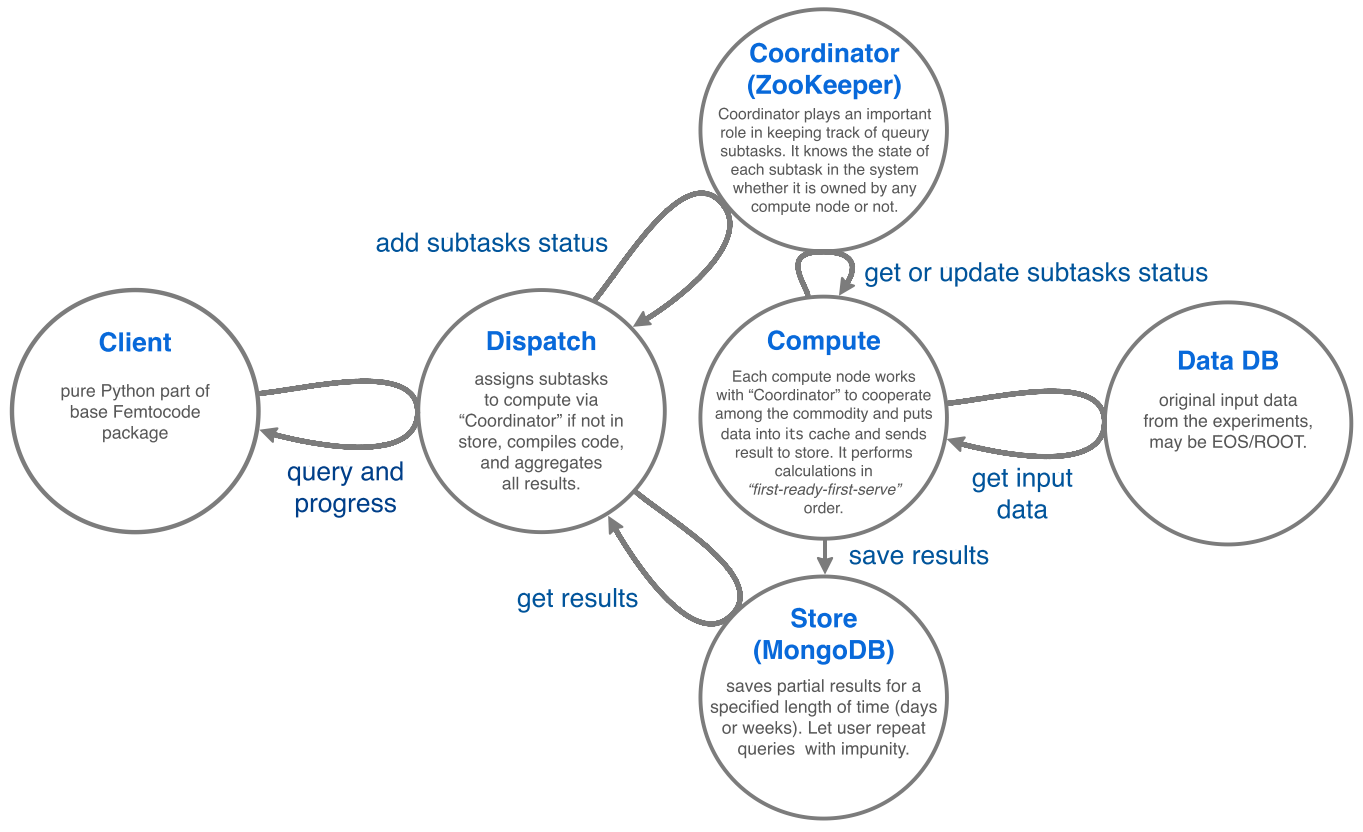
\includegraphics[width=0.75\linewidth]{distributed-layout.png}
\end{center}

\footnotetext[1]{\textcolor{blue}{\url{https://cds.cern.ch/record/2278211}}}
\footnotetext[2]{\textcolor{blue}{\url{https://github.com/JThanat/femto-mesos/tree/master}}}
\end{frame}

\begin{frame}
\begin{center}
\huge \textcolor{darkblue}{Query language}
\end{center}
\end{frame}

\begin{frame}{Femtocode}
\vspace{0.5 cm}

Femtocode\footnotemark[1] is a mini-language based on Python, but with sufficient limitations to allow SQL-like query planning.

\vspace{0.25 cm}
\begin{itemize}\setlength{\itemsep}{0.25 cm}
\item Dependent type-checking to ensure that every query completes without runtime errors.
\item Automated vectorization/GPU translation by controlling the loop structure.
\item Integrates database-style indexing with processing.
\end{itemize}

\vspace{0.25 cm}
But these are all ``2.0'' features.

\footnotetext[1]{\textcolor{blue}{\url{https://github.com/diana-hep/femtocode/}}}
\end{frame}

\begin{frame}
\begin{center}
\huge \textcolor{darkblue}{Conclusions}
\end{center}
\end{frame}

\begin{frame}{Conclusions!}
\vspace{0.5 cm}

\begin{itemize}\setlength{\itemsep}{0.5 cm}
\item AOD-to-plot in seconds {\it is possible.}
\item They're doing it in industry (but\ldots\ SQL and Java).
\item Python-based queries can be computed at single-threaded rates of 10--100~MHz by translating code, rather than deserializing data.
\item Columnar data granularity has useful consequences.
\item Prototyping distributed architecture, relying on third-party components wherever possible.
\end{itemize}
\end{frame}

%% the dream: motivation

%% existence proof: Drill (and others)

%%    * lightweight parallelization
%%    * columnar data
%%    * distributed, in-memory caching
%%    * JIT compilation, vectorization
%%    * data stay on server, only summaries come down

%% pieces we would need: (1) fast execution (2) distributed processing (3) \sout{query language} (in abstract, but focus has turned more to the above)

%% fast execution

%% not better--- best (microbenchmarks to define goal; usefulness of knowing that {\it no} improvement is possible)

%%    * running through data in CMSSW (just an example) vs an HPC-like minimal for loop in C: rate and data touched
%%    * reflects difference in design: CMSSW was {\it meant} to heavy processing on a lot of data per event (reconstruction);
%%      but this makes it a poor choice for lightweight analysis jobs
%%    * analysts mostly use it to dump data to skims, but the slower the framework is per event, the more that needs to be dumped to make it worthwhile (rich get richer)
%%    * lightweight process without persistent skim is a different ``local minimum in ease-of-use space''

%% microbenchmarks are in C, but Python + Numba is also an option: Python is good for informal scripting, developing algorithms quickly, and Numba compiles it with LLVM; runtime is indistinguishable

%% the problem with this is that most of what we want to do with our data doesn't look like simple for loops: we want to pair up particle objects, compute masses, isolations, match reco & MC, etc.; creating objects at runtime is expensive and brings us back to frameworks

%% alternative: instead of making objects at runtime, transform object-oriented code into array manipulation (EXAMPLE)

%% this is formal and general: start with type system and propagate object types through code like a compiler pass, then hand transformed code to Numba for optimization

%%    * P, L, U, R (website)

%% data are in contiguous columnar arrays, like ROOT TBranches, but remain in arrays at runtime

%%    * format allows for random access (EXAMPLE)
%%    * I'm adding TBranch --> Numpy to ROOT to do this on-the-fly (ROOT 6.12)
%%    * but also caching mechanism for more speed and flexibility: the new granularity is not files but columns

%% it's fast, but does it parallelize? yes, up to 2 GB/s per machine (memory bus becomes the bottleneck; plot shows microbenchmark on KNL to avoid memory bus and beat the bottleneck)

%% distributed processing

%% submitting a query and getting back an {\it aggregation} (histogram) is more complex than batch submission

%%    * something in the system must collect partial results from parallel subtasks and add them up
%%    * unavoidable state in the system

%% look at prior art: Hadoop, Spark, and Drill all do this, all are based on Apache Zookeeper

%%    * Zookeeper: distributed, fault-tolerant key-value store for rapidly changing configuration
%%    * ``configuration'' == who's working on what subtask, who's done, which need to be retried, etc.

%% current design (J.Thanat, summer student):

%%    * Zookeeper maintains pool of unfinished subtasks
%%    * workers attempt to claim ownership, preferably if they have input columns in cache (for data locality), but will take anything if they're not busy (to elastically duplicate cache for popular datasets)
%%    * we don't handle {\it any} mutable state ourselves (except volatile cache), no single point of failure (more lessons from industry)

%% query language

%%    * Femtocode is a mini-language based on Python, but with sufficient limitations to allow SQL-like query planning, automated vectorization/GPU translation, and database-style indexing
%%    * but these are all ``2.0'' features

%% conclusions

%%    * AOD-to-plot in seconds {\it is possible}
%%    * they're doing this in industry (but\ldots\ SQL and Java)
%%    * single-threaded kernel is operating in the MHz range (on ``Python'' code)
%%    * prototyping distributed architecture

\end{document}
